\subsection{Inheritance}
\subsubsection{Syntax}
\begin{lstlisting}[style=Csharp]
  class A //Basisklasse
  {
    int a; 
    public A(){};
    public void F(){};
  }
  
  class B:A //Unterklasse, erbt von A, erweitert A
  {
    int b, 
    public B(){};
    public void G(){};
  }
\end{lstlisting}
\begin{itemize}
  \item B erbt a und F()
  \item B fügt b und G() hinzu
  \item Konstruktoren werden nicht weiter vererbt
  \item Vererbte Methoden können überschrieben werden
  \item \textbf{Single Inheritance}: Ein Klasse kann nur von \textbf{einer}
  Basisklasse erben 
  \item Ein Klasse kann \textbf{nur} von einer Klasse erben, \textbf{nicht} von
  einem Struct
  \item Eine Klasse kann von mehreren Interfaces erben und 
  muss diese somit implementieren
  \item Structs können \textbf{nicht} von anderen Typen erben, aber sie können
  diverse Interfaces implementieren
  \item Ein Klasse \textbf{ohne} explizite Basisklasse erbt von der Klasse
  \textbf{Object}
\end{itemize}
 
\subsubsection{Zuweisungen und Type Checks}
\begin{lstlisting}[style=Csharp]
  class A{...};
  class B:A{...};
  class C:B{...};
  
  //Assignments
  A a = new A();  //Static type of a: the type specified in the declaration
                  //(here A)
                  //Dynamic type of a: the type of the object in a (here also A)
  a = new B();    //Dynamic type of a is B
  b = new C();    //Dynamic type of a is C
  
  B b = a;        //Forbidden, compilation Error
  
  //Run-time type checks
  a = new C(); 
  if(a is C)...   //True, if the dynamic type of a is C or a subclass, otherwise
                  //false
  if(a is B)...   //True
  if(a is A)...   //True, but warning because it makes no sense
  
  a = null; 
  if(a is C)...   //False: If a==null, a is T always returns false
\end{lstlisting}

\subsubsection{Checked Type Casts}
\begin{lstlisting}[style=Csharp]
  A a = new C(); 
  B b = (B) a;    //NO IDEA???
  a = null; 
  C c = (C) a;    //null can be casted to any reference tpye
  
  //With "as"
  A a = new C();  
  B b = a as B;   //NO IDEA???
  
  a = null; 
  C c = a as C;   //c == null
\end{lstlisting}

\subsubsection{Overriding Methods}
Nur \textbf{virtuelle} Methoden können ins Unterklassen überschrieben werden. 
\begin{lstlisting}[style=Csharp]
  class A
  {
    public         void F(){...} //Kann nicht ueberschrieben werden 
    public virtual void G(){...} //Kann ueberschrieben werden
  }
  
  class B:A
  {
    public          void F(){...} //Achtung: Versteckt vererbte Funktion F()
                                  //-> Benutze new
    public          void G(){...} //Achtung: Versteckt vererbte Funktion G()
                                  //-> Benutze new
    public override void G()      //Ok: Ueberschreibt vererbte Funktion G
    {
      base.G();                   //Ruft vererbte Funktion G auf
    }
  }
\end{lstlisting}
\begin{itemize}
  \item Die Eigenschaften (Signatur) der Methode müssen gleich bleiben 
  \begin {itemize}
    \item Gleiche Anzahl und Typ von Parmametern (einschliesslich Funktionstyp!)
    \item Gleiche Sichtbarkeit (public, protected\ldots)
  \end{itemize}
  \item Properties und Indexers können ebenfalls überschrieben werden (virtual,
  override)
  \item Statische Methoden können \textbf{nicht} überschrieben werden!
\end{itemize}

\subsubsection{Hiding}
Members können in einer Unterklasse als new deklariert werden. Sie verstecken
vererbte Members mit dem gleichen Namen und derselben Signatur. 
\begin{lstlisting}[style=Csharp]
  class A
  {
    public int x; 
    public void F(){...}
    public virtual void G(){...}
  }
  class B:A
  {
    public new int x; 
    public new void F(){...};
    public new void G(){...};
  }
  
  B b = new B(); 
  b.x = ...;      //Greife auf x von B zu 
  b.F();          //Rufe Funkionen F und G von B auf
  b.G(); 
  
  ((A)b).x = ..;  //Greife auf x von A zu
  ((A)b).F();     //Rufe Funktionen F und G von A auf
  ((A)b).G();     //(Obwohl der dynamische Typ von (A)b B ist!)
\end{lstlisting}
Weitere Beispiele: Siehe Folie 8 und 9 vom Foliensatz "`Inheritance"'

\subsubsection{Constructor in Subclasses}
\begin{figure}[h]
  \centering
  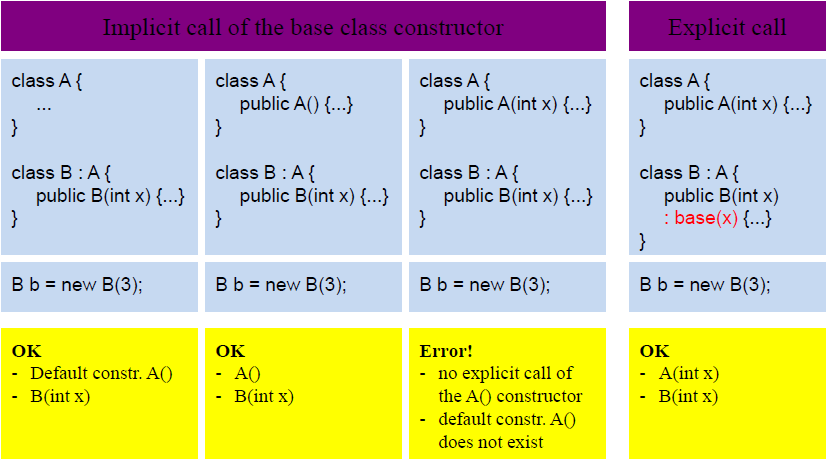
\includegraphics[height=5cm, ]{images/CSharp/ConstructorsInSubclasses}
  \caption{Konstruktoren in Unterklassen} 
\end{figure}

\subsubsection{Visibility}
\begin{itemize}
  \item \textbf{protected}: Sichtbar in der deklarierten Klasse und ihren
  Unterklassen
  \item \textbf{internal}: Sichtbar im deklarierten Assembly
  \item \textbf{protected internal}: Sichtbar in der deklarierten Klasse, ihren
  Unterklassen und im deklarierten Assembly. 
\end{itemize}

\subsubsection{Astrakte Klassen und Methoden}
\begin{itemize}
  \item Abstrakte Methoden haben \textbf{keine} Implementation
  \item Abstrakte Methoden sind implizit \textbf{virtuell}
  \item Wenn eine Klasse abstrakte Methoden (deklariert oder vererbt), muss sie
  selber \textbf{auch} abstrakt sein. 
  \item Aus einer abstrakten Klasse lassen sich \textbf{keine} Objekte
  erstellen. 
\end{itemize}
Beispiel: 
\begin{lstlisting}[style=Csharp]
  abstract class Stream
  {
    public abstract void Write(char ch);
    public void WirteString(string s)
    {
      foreach(char ch in s) 
        Write(ch); 
    }
  }
  class File:Stream
  {
    public override void write(char ch)
    {
      ...write ch to disk...
    }
  }
\end{lstlisting}

\subsubsection{Astrakte Properties und Indexers}
\begin{itemize}
  \item Indexers und Properties, welche überschrieben werden, müssen diesselben
  get und set Methoden haben wie in der Basisklasse.
\end{itemize}
Beispiel: 
\begin{lstlisting}[style=Csharp]
  abstract class Sequence
  {
    public abstract void Add(object x);             //Methode
    public abstract string Name{get;}               //Property
    public abstract object this [int i]{get; set;}  //Indexer   
  }
  class List:Sequence
  {
    public override void Add(object x){...}
    public override string Name{get{...}}
    public override object this [int i]{get{...} set{...}}
  }
\end{lstlisting}

\subsubsection{Sealed (Verschlossene) Klassen}
\begin{itemize}
  \item "`Sealed"' Klassen können nicht erweitert werden, aber sie können von
  anderen Klassen erben. 
  \item "`Override"' Methoden können individuell als "`sealed"' bezeichnet
  werden.
  \item Gründe:
  \begin{itemize}
    \item Sicherheit
    \item Effizienz
  \end{itemize}
\end{itemize}
Beispiel: 
\begin{lstlisting}[style=Csharp]
  sealed class Account:Asset
  {
    long val; 
    public void Deposit(long x){...}
    public void Withdraw(long x){...}
    ...
  }
\end{lstlisting}

\subsubsection{Basisklasse System.Object}
Oberste Basisklasse:
\begin{lstlisting}[style=Csharp]
class Object
{
  protected object      MemberwiseClone(){...}
  public Type           GetType(){...}
  public virtual bool   Equals(object o){...}
  public virtual string ToString(){...}
  public virtual int    GetHashCode(){...}
}
\end{lstlisting}
Direkt verwendbar: 
\begin{lstlisting}[style=Csharp]
class Object
{
  Type t = x.GetType();  //Returns a type descriptor
  object copy = x.MemberwiseClone();  //Does a shallow copy (protected method!)
}
\end{lstlisting}
Überschreibbar in Unterklassen: 
\begin{lstlisting}[style=Csharp]
  x.Equals(y)                 //Compare values of x and y
  y.ToString()                //Should return a string representation of x
  int code = x.GetHashCode(); //Should return a hashcode for x
\end{lstlisting}

Beispiel für Objekte und Überladen siehe Folien 16 und 17
